%!TEX root = ./template-skripsi.tex
%-------------------------------------------------------------------------------
%                            BAB II
%               TINJAUAN PUSTAKA DAN DASAR TEORI
%-------------------------------------------------------------------------------

\chapter{TINJAUAN PUSTAKA DAN DASAR TEORI}                

\section{Tinjauan Pustaka}
  Dalam beberapa tahun terakhir perkembangan teknologi sangat lah pesat, terutama teknologi perangkat lunak.Perkembangan yang pesat ini disebabkan oleh berbagai faktor, termasuk peningkatan kebutuhan akan aplikasi yang lebih canggih dan kompleks, serta kemajuan dalam metode pengembangan perangkat lunak itu sendiri.Dalam menghadapi kompleksitas dan kebutuhan yang semakin tinggi, banyak organisasi atau perusahaan yang beralih dan menggunakan pendekatan microservices dalam pengembangan perangkat lunak.

  % Microservices adalah pendekatan pengembangan perangkat lunak di mana sistem dibangun sebagai kumpulan layanan kecil yang independen. Setiap layanan berfungsi sebagai unit yang terisolasi dan memiliki tanggung jawab tersendiri dalam menjalankan fungsionalitas tertentu. Pendekatan ini berbeda dengan pendekatan monolitik yang mengembangkan sistem sebagai satu entitas tunggal.

  Salah satu tantangan yang dihadapi dalam penggunaan microservices adalah kesulitan dalam mengetahui keadaan sistem secara menyeluruh. Error yang terjadi pada suatu sistem microservices dapat disebabkan oleh banyak faktor dikarenakan tiap request yang masuk akan melewati banyak layanan yang saling terkait. Oleh karena itu, dibutuhkan sebuah metode yang dapat membantu dalam memahami dan menganalisa perilaku sebuah sistem microservices. Salah satu metode yang dapat digunakan adalah distributed tracing.

  Terdapat beberapa penelitian yang dilakukan untuk mengatasi permasalahan tersebut. diantaranya, penelitian yang dilakukan Benjamin H. Sigelman et al yang mengembangkan sebuah tracing sistem bernama Dapper untuk mengatasi permasalahan dan tantangann dalam memonitoring dan memahami perilaku sebuah sistem terdistribusi berskala besar di sistem Google. Penelitian ini membahas betapa sulit dalam mendiagnosis permasalahan performa pada sistem terdistribusi dimana sebuah request akan melewati banyak servis dan komponen sehingga dibutuhkan sebuah infrastruktur tracing untuk mengambil dan menganalisa data terkait alur request tersebut. Dapper adalah solusi yang dikembangkan oleh Google, sebuah infrastruktur pelacakan terdistribusi yang dapat mengumpulkan informasi dari berbagai servis yang terlibat dalam proses sebuah request. Sebuah request yang masuk akan menghasilkan sebuah pohon trace dimana setiap node pada pohon trace tersebut disebut span yang merepresentasikan unit kerja yang dilakukan. Pada setiap pohon trace akan terdapat annotation yang berisi informasi yang memberikan konteks mengenai kejadian yang terjadi pada span tersebut.Dapper menggunakan metode sampling dalam mengumpulkan trace alih-alih mengumpulkan semua trace dari request yang terjadi, hal ini dilakukan untuk mengurangi dampak terhadap performa pada microservices. Berdasarkan penelitian tersebut penerapan tracing pada sistem terdistribusi dapat membantu dalam memahami dan menganalisa perilaku sebuah sistem terdistribusi.

  Clement Casse et al melakukan penelitian dengan menggunakan distributed tracing untuk mengetahui penggunaan resource yang tidak efisien di aplikasi cloud. Penelitian ini fokus pada pengumpulan informasi pada microservices dan memodelkannya menjadi sebuah hierarchical model graph. Penelitian ini melakukan implementasi pada sebuah microservices aplikasi perbelanjaan yang dideploy pada sebuah cluster kubernetes yang terdiri dari 4 nodes dan 2 zones dan menggunakan opentelemetry untuk mengumpulkan data tracing. Hasil dari penelitian ini menunjukan bahwa model yang digunakan dapat mengetahui penggunaan resource cloud yang tidak efisien. 

  Menurut penelitian yang dilakukan oleh Putu Napoleon Krishna Bayu, log yang dihasilkan pada server yang memiliki lokasi secara terpisah tidak dapat lagi dimanfaatkan untuk mengetahui keadaan sistem secara efisien dikarenakan karakteristiknya yang semakin menyerupai big data dalam hal kecepatan pembuatan log, besaran volume log, dan variasi struktur log. Oleh karena itu dibutuhkan suatu solusi yaitu log management yang dapat menyimpan dan mengelola log secara terpusat. Log management terdiri dari beberapa tahapan yaitu pembuatan, pengumpulan, transformasi, penyimpanan, analysis dan archival.Penelitian ini menggunakan Elastic Stack yang merupakan produk open-source yang dikembangkan oleh elastic yaitu Elasticsearch, Logstash, dan Kibana. Elasticsearch digunakan sebagai database untuk menyimpan log, Logstash digunakan sebagai agen pengumpul data log, dan Kibana digunakan sebagai platform untuk visualisasi data log yang telah disimpan. Hasil dari penelitian yang dilakukan adalah berhasil mengimplementasikan log monitoring system yang menjalankan tahapan-tahapan log management dengan menggunakan Elastic Stack sehingga keadaan dua buah server dapat dikelola dan dimonitor secara terpusat.

  Kemudian, penelitian yang dilakukan oleh Guntoro Yudhy Kusuma et al yang melakukan perancangan sistem monitoring performa aplikasi menggunakan Opentelemetry dan Grafana Stack. Aplikasi monitoring yang dirancang berperan untuk mengumpulkan data telemetri berupa metrics dan traces dari sebuah sistem REST API yang diinstrumentasi menggunakan sebuah kerangka kerja sumber terbuka Opentelemetry. Data telemetri metrics yang telah dikumpulkan akan dikirim menuju sebuah alat alerting dan monitoring Prometheus sedangkan data telemetri traces akan dikirim menuju sistem backend Jaeger. Prometheus dan Jaeger kemudian diintegrasikan ke Grafana sebagai alat visualisasi data telemetri. Hasil dari penelitian ini menunjukan bahwa rancangan sistem monitoring berjalan dengan baik dengan beberapa kelemahan diantaranya penurunan jumlah throughput secara rata-rata sebesar 23,32\% dan kenaikan secara rata-rata sebesar 22,80\% pada request latency. 
  
  Pada Kubecon North America 2021 yang merupakan sebuah konferensi untuk pengembang Kubernetes, Juraci Paixao Kroehling menjelaskan bagaimana saja deployment pattern untuk Opentelemetry Collector. Terdapat dua pattern untuk melakukan deployment Opentelemetry Collector pada Kubernetes yaitu: 
  \begin{enumerate}
    \item Deployment menggunakan Sidecar
    
    Sidecar pada Kubernetes merupakan sebuah container yang berjalan bersama container utama pada sebuah pod. pada pattern ini Opentelemetry Collector akan dijalankan sebagai sebuah sidecar bersamaan dengan kontainer utama (aplikasi utama). Kontainer utama akan mengirimkan data telemetri menuju sidecar Opentelemetry Collector yang kemudian sidecar tersebut akan mengirimkan data telemetri tersebut ke external collector seperti pada gambar 2.2.1.

    \begin{figure}[H]
      \centering
        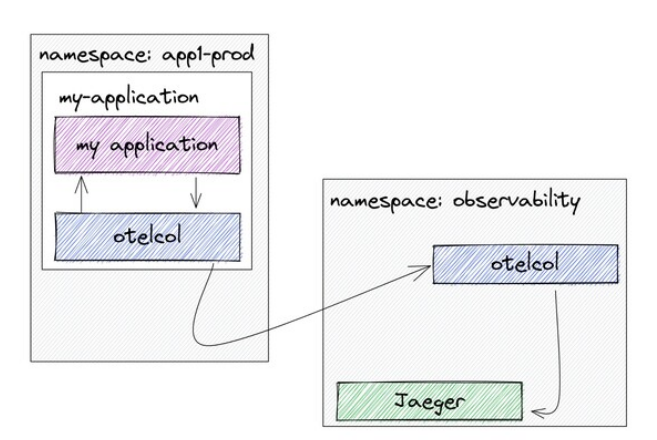
\includegraphics[scale=0.8]{gambar/sidecar-pattern}
        \caption{Deployment Opentelemetry Collector dengan sidecar.}
        \label{otel-collector-sidecar}
    \end{figure}
    
  \item Deployment menggunakan DaemonSet
  
  Berbeda dengan sidecar, DaemonSet menjalankan Opentelemetry Collector pada setiap node. Cara kerja dari pattern ini adalah setiap pod yang berada pada satu node akan mengirimkan data telemetri menuju OpenTelemetry Collector pada node tersebut yang kemudian akan mengirimkan data telemetri tersebut ke external collector seperti pada gambar 2.2

  \begin{figure}[H]
    \centering
      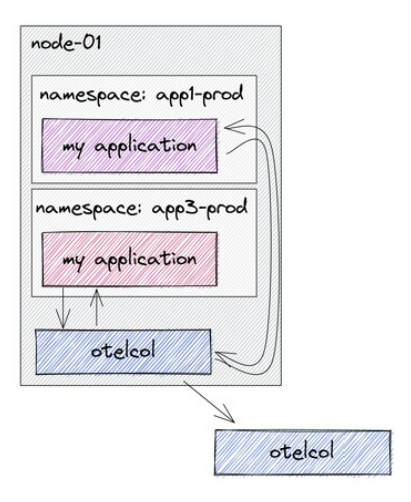
\includegraphics[scale=0.8]{gambar/daemonset-pattern}
      \caption{Deployment Opentelemetry Collector dengan daemonset.}
      \label{otel-collector-daemonset}
  \end{figure}

  \end{enumerate}

  Rolando Brondolin et al melakukan penelitian dengan mengembangkan sebuah pendekatan Black-box monitoring untuk mengukur runtime performa pada microservices. Penelitian ini menggunakan teknologi extended Berkeley Packet Filter (eBPF) yang digunakan untuk mengumpulkan data terkait performa aplikasi, penggunaan power, dan aktivitas network pada setiap docker container, kubernetes host dan physical host. eBPF merupakan sebuah teknologi yang memungkinkan penulis dapat membuat program yang berjalan di level kernel dengan aman, Dengan eBPF penulis dapat membuat sebuah program yang bertujuan untuk mengekstrak data metrics yang dibutuhkan untuk pengukuran performa aplikasi. Peneliti membuat dua eBPF program berbeda dengan tujuan masing-masing untuk mengumpulkan data performa dan data network. Kedua program tersebut bereaksi pada Linux tracepoint dan Kprobe yang khusus pada data yang ingin dikumpulkan. Ketika eBPF VM menerima event dari linux kernel, event tersebut akan dikirimkan menuju program eBPF yang telah dibuat sesuai dengan jenis event kemudian hasil dari program tersebut akan dikirim dan disimpan pada hash map yang dapat diakses oleh user-space agen. kemudian, user-space agen akan mengirimkan data yang telah dikumpulkan menuju remote backend.

\section{Landasan Teori}
  \subsection{Microservices}
  Microservices merupakan sebuah aristektur perangkat lunak yang terdiri dari banyak servis yang independen. Setiap servis mengenkapsulasi fungsi sebuah proses tertentu dan saling berkomunikasi melalui jaringan\cite{BuildingMicroservices}. Sebagai contoh sebuah aplikasi toko online yang terdiri dari beberapa servis yaitu inventory, account, dan shipping seperti pada gambar 2.1. 
  
  \begin{figure}[H]
    \centering
      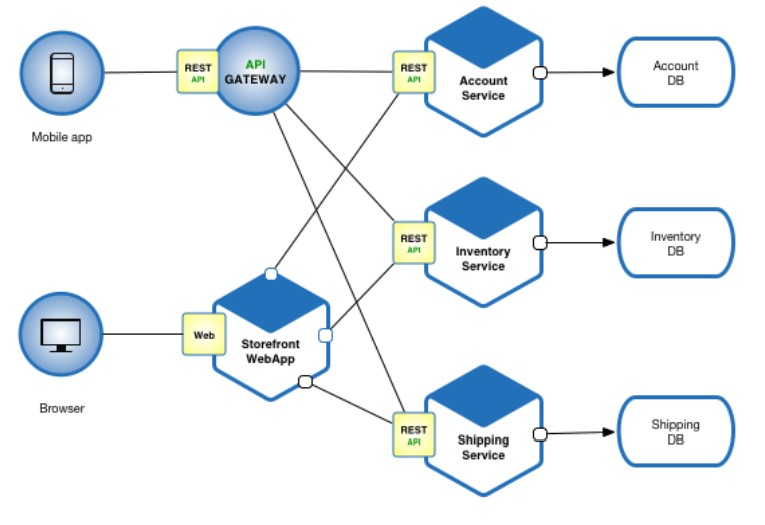
\includegraphics[scale=0.8]{gambar/microservices_architecture}
      \caption{Arsitektur microservices toko online.}
      \label{microservices}
  \end{figure}

  \subsection{Docker}
  Docker merupakan sebuah teknologi sumber terbuka yang berjalan di windows atau linux yang membantu dalam membuat, mengatur, dan melakukan orkestrasi kontainer. Kontainer merupakan sebuah paket ringan yang berisi kode perangkat lunak, environment serta dependensi lainnya. Kontainer memungkinkan sebuah aplikasi untuk berjalan di lingkungan yang terisolasi pada sebuah host seperti pada gambar 2.2.

  \begin{figure}[H]
    \centering
      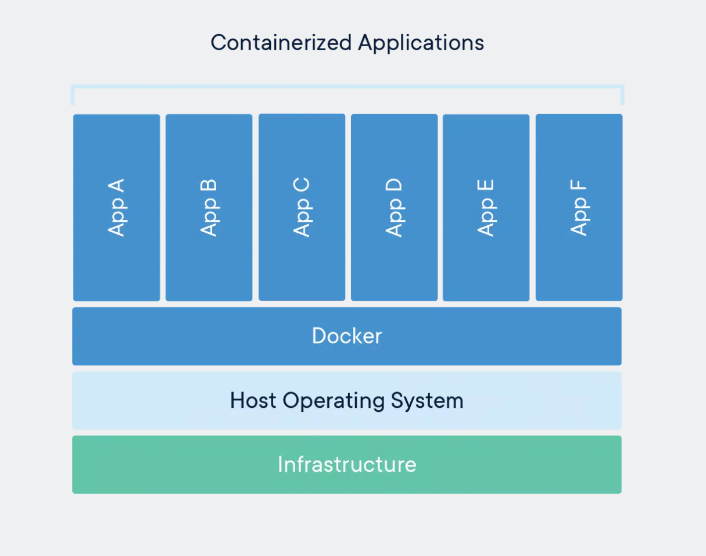
\includegraphics[scale=0.5]{gambar/docker-container}
      \caption{Kontainer yang berjalan pada sebuah host.}
      \label{containerized}
  \end{figure}

  \subsection{Kubernetes}
  Kubernetes merupakan sebuah platform sumber terbuka yang merupakan bagian dari Cloud Native Computing Foundation (CNCF). Kubernetes digunakan untuk melakukan manajemen container secara otomatis. Kubernetes memiliki kemampuan diantaranya load balancing, manajemen storage, otomasi rollouts dan rollback, pembatasan resource container, self-healing, dan manajemen konfigurasi\cite{Kubernetes}. 

  Sebuah kubernetes cluster terdiri dari beberapa node. Sebuah node dapat merupakan sebuah linux host yang berjalan baik pada mesin fisik atau virtual. Terdapat dua jenis node pada kubernetes yaitu control plane node dan worker node\cite{kubernetesNigelPoulton}. Sebuah control plane node beperan untuk mengatur dan mengontrol worker node sedangkan worker node berperan untuk menjalankan aplikasi yang berjalan pada sebuah kontainer sperti pada gambar.

  \begin{figure}[H]
    \centering
      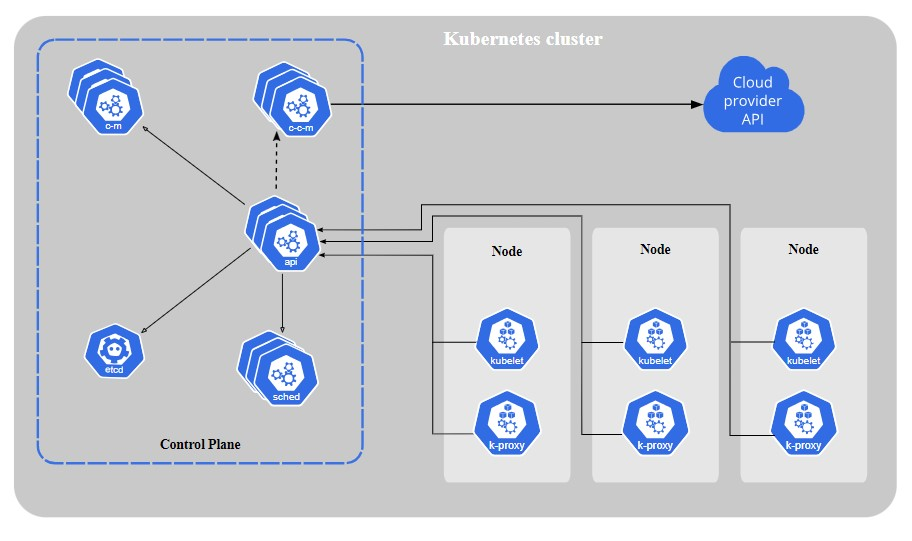
\includegraphics[scale=0.7]{gambar/kubernetes-component}
      \caption{Komponen-komponen pada kubernetes cluster.}
      \label{kubernetes-component}
  \end{figure}

  \subsection{Minikube}
  Minikube merupakan sebuah tool yang digunakan untuk menjalankan sebuah kubernetes cluster pada sebuah host lokal yang tersedia untuk Linux, macOS, dan Windows. Minikube bekerja dengan cara membuat sebuah virtual machine yang berisi sebuah single-node kubernetes cluster. Minikube dapat digunakan untuk melakukan eksperimen pada kubernetes atau untuk melakukan development aplikasi yang akan di deploy pada sebuah cluster kubernetes\cite{Minikube}.

  \subsection{Distributed Tracing}
  Tracing merupakan suatu metode untuk mengetahui serangkaian kejadian atau event yang terjadi pada sebuah request aplikasi. Sebuah tracing dikatakan distributed apabila dalam request tersebut melibatkan atau melewati beberapa proses atau mesin atau jaringan yang berbeda. Sebuah request digambarkan sebagai trace yang terdiri dari beberapa span, span tersebut merupakan unit terkecil kejadian yang terjadi pada sebuah trace. Gambar sebuah trace dapat dilihat pada gambar 2.4.
  
  \begin{figure}[H]
    \centering
      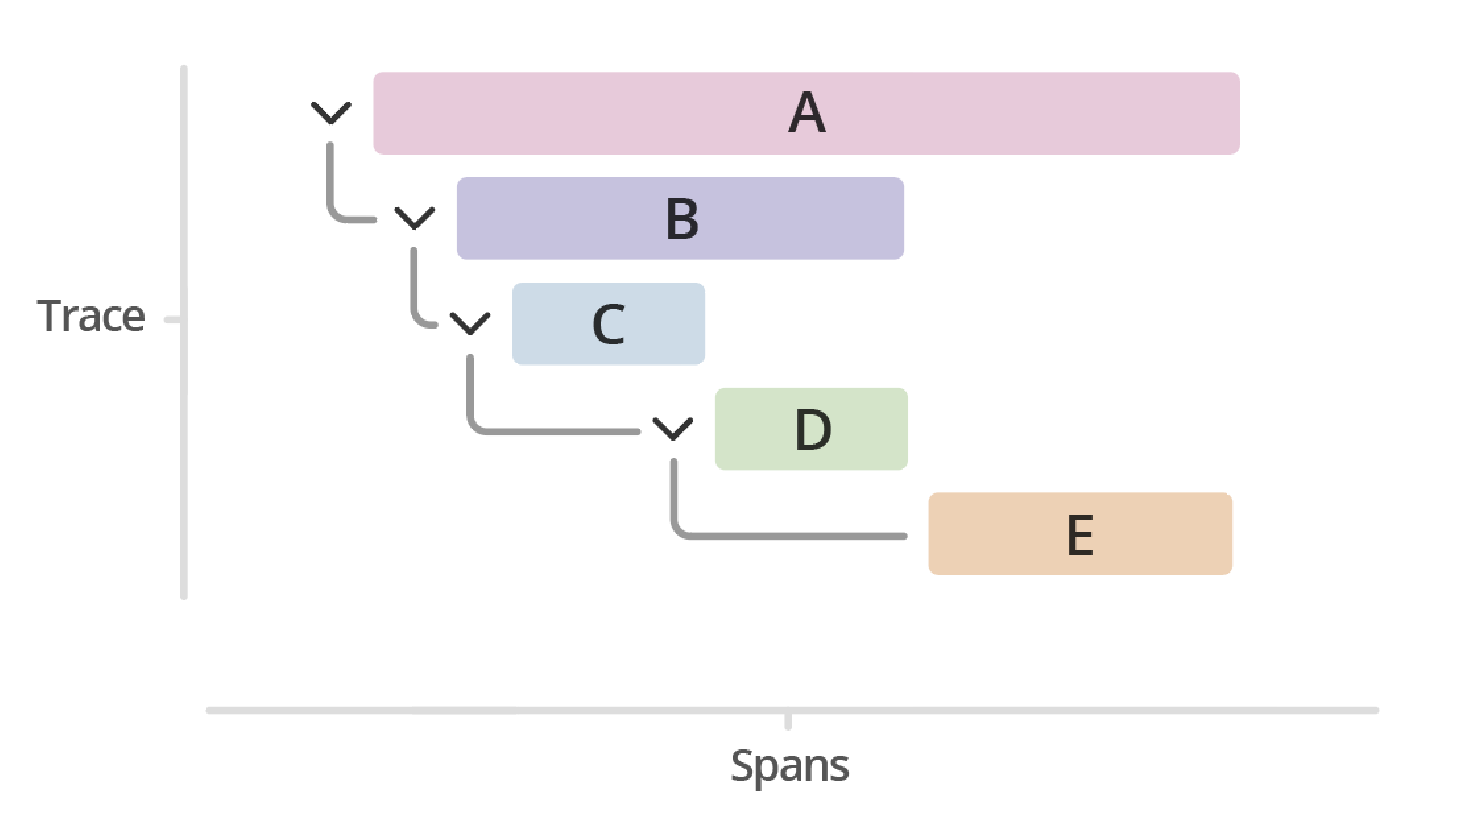
\includegraphics[scale=0.6]{gambar/traces-spans}
      \caption{Trace.}
      \label{Trace}
  \end{figure}

  Distributed tracing bekerja dengan cara menginstrumentasi aplikasi sehingga ketika sebuah request masuk aplikasi akan membuat sebuah traceID kemudian traceID tersebut akan dikirimkan ke setiap proses yang dilalui oleh request tersebut. Setiap proses akan membentuk sebuah span dengan spanID. Span akan menyimpan informasi seperti waktu mulai dan selesai, durasi, dan metadata terkait. Kemudian, trace dan span yang telah dibuat akan digabungkan sesuai urutannya oleh sebuah sistem atau platform distributed tracing.

  \subsection{OpenTelemetry}
  Opentelemetry merupakan observability framework yang bersifat sumber terbuka dan merupakan projek dari CNCF. Opentelemetry menyediakan standar, tools, APIs, dan SDKs yang dapat digunakan untuk instrumentasi, menghasilkan, mengumpulkan, dan mengeskport data telemetri (metrics, logs, traces) untuk membantu dalam analisis performance pada aplikasi. Opentelemetry besifat vendor-agnostic yang berarti dapat digunakan di bahasa dan teknologi banyak teknologi\cite{WhatIsOpentelemetry}.

  Opentelemetry terdiri dari beberapa komponen, yaitu

  \begin{enumerate}
    \item API and SDK\\
    Opentelemetry sudah menyediakan API (application programming interface) dan SDK (Software Development Kit) untuk berbagai macam bahasa pemrograman sehingga dapat membantu untuk melakukan instrumentasi pada aplikasi dengan berbagai bahasa untuk menghasilkan metrics dan tracing telemetri.
    \item OpenTelemetry Collector\\
    Opentelemetry collector merupakan sebuah implementasi yang bersifat vendor-agnostic untuk melakukan penerimaan, pemrosesan, dan mengirimkan data telemetri. dengan opentelemetry collector data telemetri dapat dikirimkan ke berbagai backend tools seperti Jaeger, Prometheus, Zipkin, dan lain-lain\cite{OtelCollector}. Arsitektur dari opentelemetry collector dapat dilihat pada gambar 2.5.

      \begin{figure}[H]
        \centering
          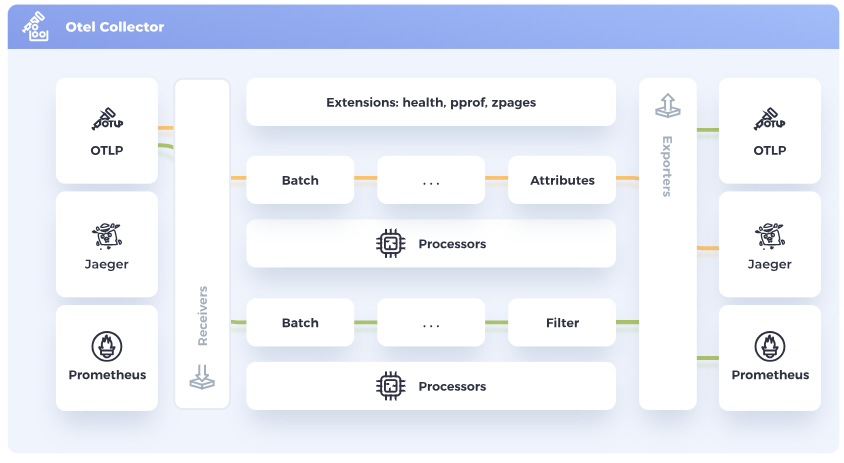
\includegraphics[scale=0.7]{gambar/otel-collector}
          \caption{Arsitektur Opentelemetry collector.}
          \label{Arsitektur Opentelemetry collector.}
      \end{figure}
      
    Gambar .... merupakan contoh data telemetri traces dengan standar Opentelemetry.

    \begin{figure}[H]
      \centering
        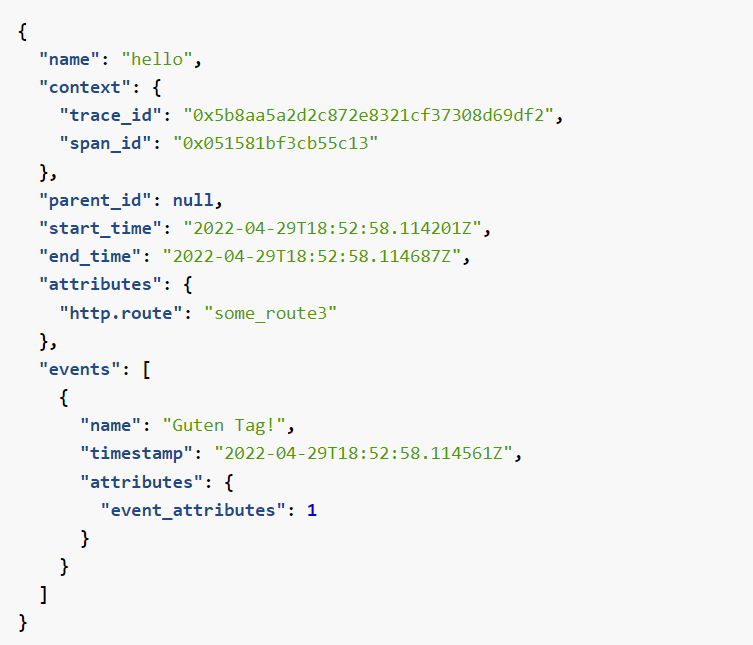
\includegraphics[scale=0.8]{gambar/otel-data-traces}
        \caption{OpenTelemetry data trace.}
        \label{Otel data trace.}
    \end{figure}

    \item OpenTelemetry Protocol\\
    OTLP merupakan protokol untuk mentransmisikan traces, metrics, dan logs telemetri. OTLP membantu Opentelemetry untuk mengirimkan data 13
    ke banyak backend tools. OTLP mengatur bagaimana encoding, transport, dan mekanisme pengiriman data.
  \end{enumerate}
  Bagaimana Opentelemetry bekerja dapat dilihat pada gambar Sebuah aplikasi akan menggunakan API dan SDK Opentelemetry untuk menginstrumentasi data telemetri kemudian data tersebut di proses sebelum di export/kirim menuju collector dan dari collector akan diexport menuju backend tools.

  \begin{figure}[H]
    \centering
      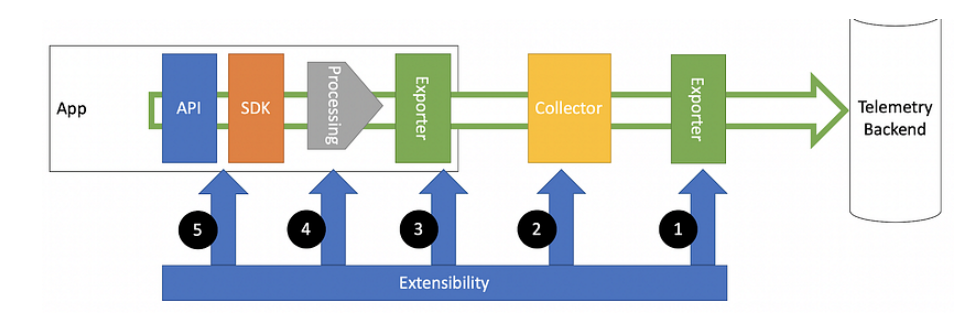
\includegraphics[scale=0.7]{gambar/otel-working}
      \caption{Alur kerja Opentelemetry}
      \label{Alur kerja Opentelemetry.}
  \end{figure}

  \subsection{REST API}
  Application Programming Interface atau API merupakan sekumpulan kode atau aturan yang mengizinkan dua aplikasi saling berkomunikasi. Salah satu jenis API ada REST API. REST (Representational State Transfer) API merupakan arsitektur API dimana komunikasi yang terjadi antar dua aplikasi bersifat stateless dan menggunakan protokol HTTP atau HTTPS. REST API menggunakan HTTP method seperti GET, POST, PUT, dan DELETE dan menggunakan JSON sebagai format penerimaan atau pengiriman data.

  \begin{figure}[H]
    \centering
      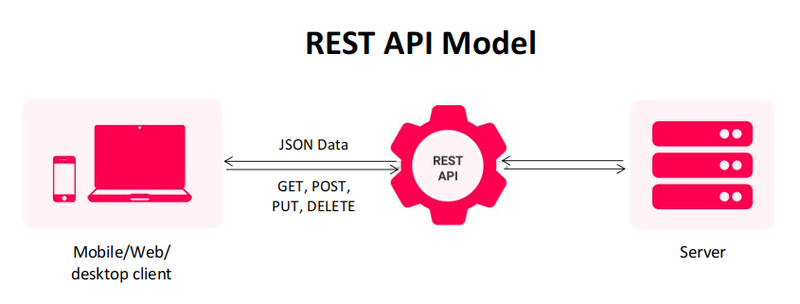
\includegraphics[scale=0.5]{gambar/rest-api}
      \caption{Alur kerja REST API.}
      \label{Alur kerja REST API.}
  \end{figure}

  Gambar 2.7 merupakan alur kerja dari sebuah REST API dimana sebuah klien melakukan request dengan method GET/POST/PUT/DELETE kemudian request tersebut akan diterima oleh server dan server akan mengirimkan response sesuai dengan request yang diterima dalam bentuk JSON seperti pada gambar .

  \begin{figure}[H]
    \centering
      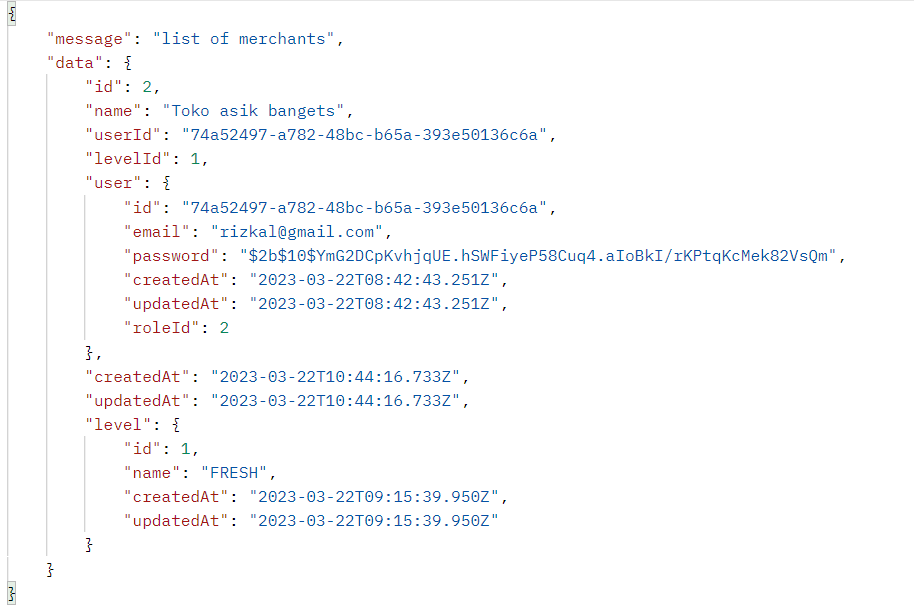
\includegraphics[scale=0.7]{gambar/json-example}
      \caption{Format data JSON.}
      \label{Format data JSON.}
  \end{figure}
  
  \subsection{Load Testing}
  Load testing merupakan salah satu jenis pengujian pada aplikasi perangkat lunak. Load testing menguji perangkat lunak dengan memberikan beban yang biasanya berupa request ke aplikasi untuk melihat apakah aplikasi tersebut mampu mengatasi beban tersebut dengan baik. Ada banyak tools sumber terbuka untuk melakukan load testing seperti k6, JMeter, Locust, dan lain-lain.